\chapter{Cristalli}
\label{ch:cristalli}
I solidi vengono descritti da strutture ordinate dette strutture cristalline: La prima volta che si ebbe l'intuizione che c'è dell'ordine nella struttura della materia fu grazie alla diffrazione dei Raggi X. Se un raggio X che trapassa un materiale alla sua uscita presenza di un reticolo di diffrazione implica che c'è una struttura ben precisa al suo interno. 
\begin{figure} [H]
	\centering
	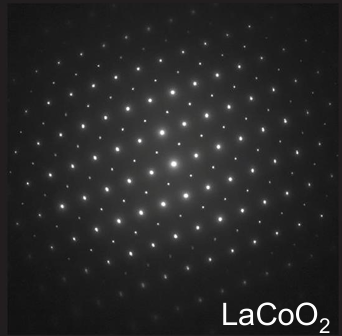
\includegraphics[width=0.15\textwidth]{images/2-Cristalli/xraydiff.png}
	\caption{qui si osserva il reticolo di diffrazione del \ce{LaCO2} da cui si deduce che in realtà la struttura è più complicata poiché ho dei punti più luminosi di altri}
	\label{fig:xraydiff}
\end{figure}

In natura gli elementi si presentano in diverse strutture e ce ne possono essere di diversi tipi: 
\begin{figure} [H]
	\centering
	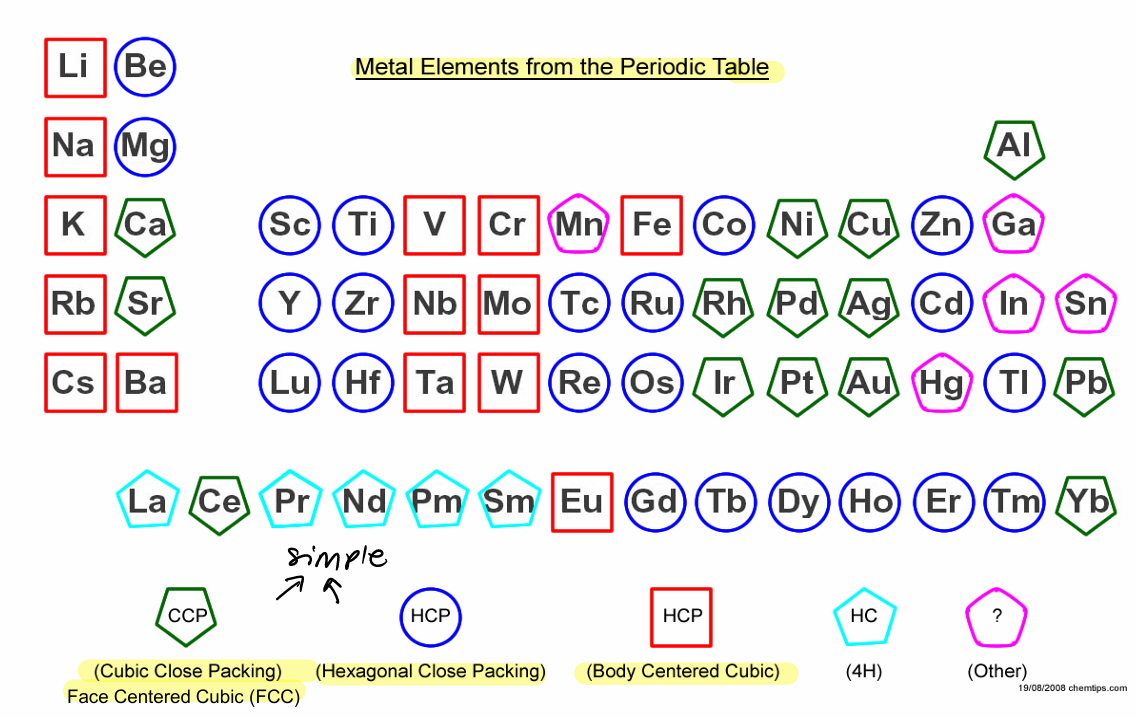
\includegraphics[width=0.55\textwidth]{images/2-Cristalli/strutturacrist.png}
	\caption{}
	\label{fig:strutturacrist}
\end{figure} 

\section{Reticolo di Bravais}
Un concetto fondamentale nella descrizione di qualsiasi tipo di solido cristallino è quello del \textbf{reticolo di Bravais}. Ci sono 2 possibili definizioni equivalenti per il reticolo di Bravais e sono:
\begin{itemize}
	\item Un reticolo di Bravais è un array infinito di punti discreti con posizioni e orientazioni precise che sono esattamente le stesse a prescindere dal punto in cui l'array viene osservato.
	\item Un reticolo di Bravais (tridimensionale) consiste in tutti i punti che possono descritti con vettore di posizione R della forma: \begin{equation} \vec{R} = n_1 \vec{a}_1 + n_2\vec{a}_2 + n_3 \vec{a}_3 \end{equation} dove $a_1,a_2,a_3$ sono 3 vettori qualsiasi che non appartengono allo stesso piano (non complanari) ed $n_1,n_2,n_3$ sono degli interi. Il punto $\sum_i n_i a_i$ si raggiunge facendo $n_i$ passi di lunghezza $a_i$ nella direzione i. 
\end{itemize}
Se sommo due elementi del reticolo di Bravais ottengo ancora un elemento del reticolo di Bravais: $R \in BL, \ R' \in BL \implies R + R' \in BL, \ R-R' \in BL$ \\
\begin{figure} [H]
	\centering
	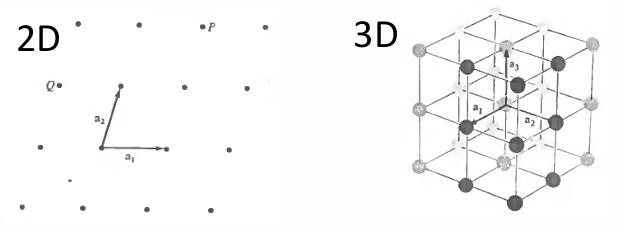
\includegraphics[width=0.55\textwidth]{images/2-Cristalli/reticoliB.png}
	\caption{Questi sono esempi di reticoli di Bravais: nel caso 2D avendo $a_1$ e $a_2$ e nel caso 3D avendo $a_1, a_2$ e $a_3$ posso ricostruire l'intero cristallo}
	\label{fig:reticoliB}
\end{figure} 

Un'altra definizione equivalente di reticolo di Bravais è: un set discreto di vettori (non appartenenti allo stesso piano) invarianti per somma e sottrazione.
\begin{figure} [H]
	\centering
	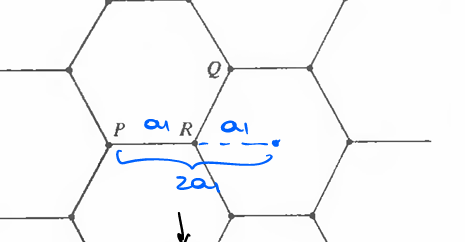
\includegraphics[width=0.55\textwidth]{images/2-Cristalli/nonBL.png}
	\caption{In figura è riportato un esempio del reticolo cristallino del Grafene che NON è un reticolo di Bravais, questo perché se al segmeto PR sommo a, che dovrebbe essere il passo del reticolo raggiungo una zona in cui non è presente nessun punto (nessun atomo), se fosse un reticolo di Bravais con $2a$ dovrei raggiungere un punto del reticolo di Bravais perché dovrei riuscire a ricostruire tutto il reticolo cristallino}
	\label{fig:nonBL}
\end{figure}

Ho una scelta infinita di vettori $a$, che vengono denominati \textbf{vettori primitivi} per definire un reticolo di Bravais, ma alcuni sono meglio di altri, vedremo le diverse scelte per diversi tipi di reticoli di Bravais.

\subsection{Cubo Semplice}
\begin{figure} [H]
	\centering
	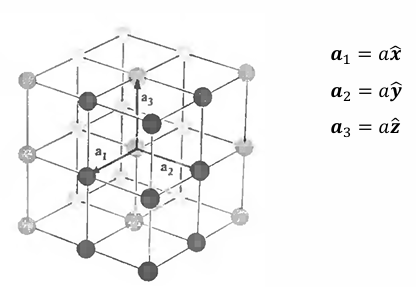
\includegraphics[width=0.55\textwidth]{images/2-Cristalli/cubosemplice.png}
	\caption{i vettori primitivi sono 3 vettori perpendicolari}
	\label{fig:cubosemplice}
\end{figure} 

\subsection{Body Centered Cube (BCC)}
\begin{figure} [H]
	\centering
	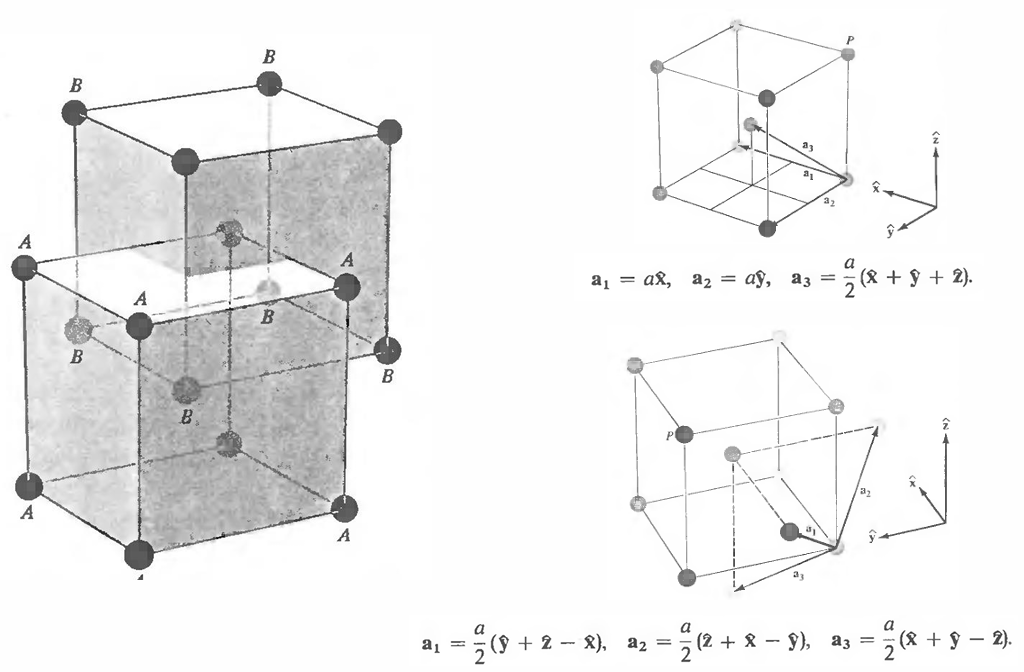
\includegraphics[width=0.9\textwidth]{images/2-Cristalli/BCC.png}
	\caption{}
	\label{fig:BCC}
\end{figure} 
Il cubo a corpo centrato è formato da due reticoli cubici compenetranti, in pratica è un cubo con un atomo al centro, dalla Figura \ref{fig:dimBCC} si dimostra che il BCC è un reticolo di Bravais. 
\begin{figure} [H]
	\centering
	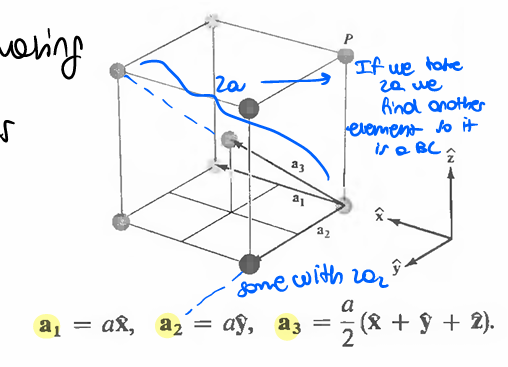
\includegraphics[width=0.5\textwidth]{images/2-Cristalli/dimBCC.png}
	\caption{Prendendo due volte il vettore $a_3$ incontro un atomo del cristallo quindi è per questo che è un reticolo di Bravais}
	\label{fig:dimBCC}
\end{figure} 
I metalli che presentano una struttura a BCC sono i metalli più duri, la presenza di quell'atomo centrale nel cubo crea frizione, i metalli deformabili invece sono formati da strati impilati l'uno sopra l'altro quindi molto più facili da deformare o spezzare (elementi di questo tipo sono Ba, Cr, Cs, Fe, K).

\subsection{Face Centered Cube (FCC)}
In questo caso invece ho un atomo al centro delle facce di ogni cubo. La struttura è piramidale con strati successivi orientati in maniera alternata.
\begin{figure}[H]
	\centering
	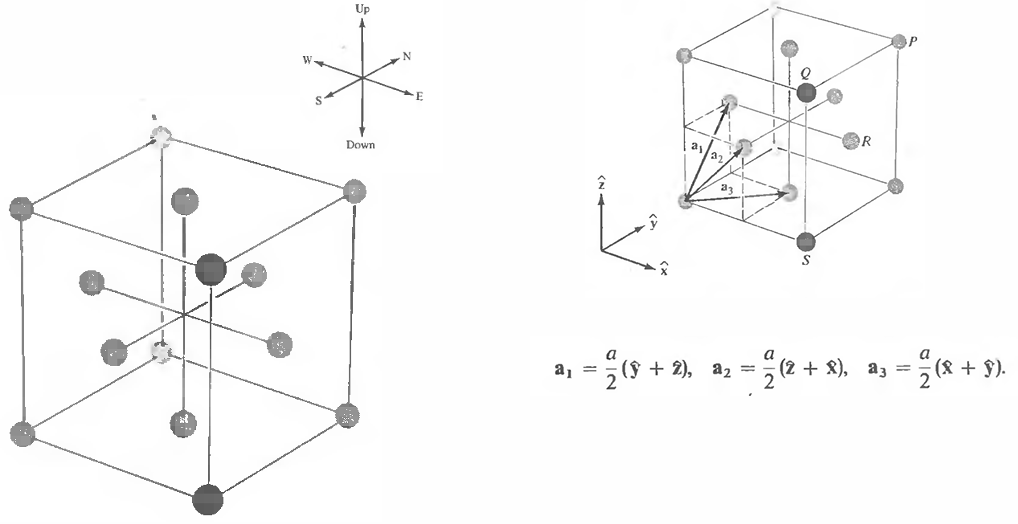
\includegraphics[width=0.9\textwidth]{images/2-Cristalli/FCC.png}
	\caption{}
	\label{fig:FCC}
\end{figure} 
Sono gli elementi più facili da deformare (gli elementi di questo tipo sono: Ar, Ag, Al, Au, Ca, Ce, $\beta$-Co, Cu).



\subsubsection{Coordination Number}
Il \textbf{coordination number} è il numero di primi vicini che ogni atomo ha all'interno di un certo cristallo, per esempio per il cubo semplice sono 6 per il BCC 8 e per l'FCC 12.

\subsection{Cella Primitiva Unitaria}
Una \textbf{cella primitiva unitaria} è una porzione di spazio (un volume) che se traslata lungo i vettori del reticolo di Bravais riempie tutto lo spazio senza lasciare buchi o sovrapponendosi a qualcosa. Anche in questo caso ci sono più scelte possibili di cella primitiva ma ce ne sono alcune che sono più importanti di altre. Le diverse scelte di cella primitiva però dovranno avere lo stesso volume. 
\\~\\
Una cella primitiva molto importante è la \textbf{cella di Wigner Seitz} che è una cella primitiva che mantiene la simmetria locale del cristallo. La WSC di un punto del reticolo è data dalla regione di spazio più vicina a quel punto rispetto a qualsiasi altro punto del reticolo. In Figura \ref{fig:WSC} è mostrato un esempio di una cella WSC.
\begin{figure} [H]
	\centering
	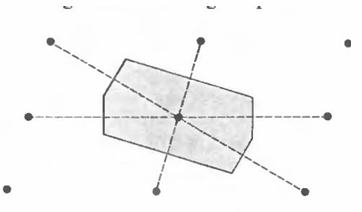
\includegraphics[width=0.5\textwidth]{images/2-Cristalli/WSC.png}
	\caption{Per costruire una cella di Wigner Seitz taglio a metà le linee che connettono tutti i gli altri atomi all'atomo centrale}
	\label{fig:WSC}
\end{figure} 

La WSC del BCC è un ottaedro troncato e quella dell'FCC è un dodecaedro rombico, la simmetria della WSC è correlata a quella del reticolo perché infatti nel caso del BCC dove abbiamo come numero di coordinazione 8 (quindi 8 primi vicini) abbiamo un ottaedro mentre nel caso dell'FCC che ha come numero di coordinazione 12 abbiamo un dodecaedro.

\section{Struttura cristallina, reticoli con base}
Una struttura cristallina non è un reticolo di Bravais e consiste in copie identiche della stessa unità fisica, chiamata \textbf{base}, localizzata nei punti di un reticolo di Bravais. \\
Un atomo è al centro del reticolo di Bravais e descrivo l'altro rispetto al reticolo quindi la sua posizione sarà $\Vec{R}+d$. In pratica colleziono coppie di atomi e questi due possono essere descritti da un reticolo di Bravais. La posizione dell'atomo è descritta da:
\begin{itemize}
	\item dal centro della cella unitaria descritta da un reticolo di Bravais $\implies \Vec{R}$
	\item dalla posizione relativa degli atomi all'interno della cella unitaria $\implies \Vec{R} + \Vec{d}$
\end{itemize}
\begin{figure} [H]
	\centering
	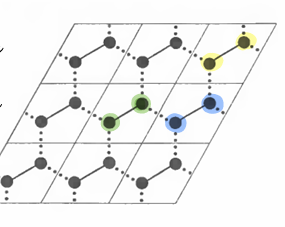
\includegraphics[width=0.5\textwidth]{images/2-Cristalli/struttcristall.png}
	\caption{}
	\label{fig:struttcristall}
\end{figure} 
\subsection{Strutture a diamante}
Nelle figure \ref{fig:diamantebase1} e \ref{fig:diamantebase2} è riportata una tipologia di cristalli con base che sono i cristalli con \textbf{struttura a diamante} che sono degli FCC con base, inoltre i siti atomici hanno tutti una struttura tetraedrica ad ibridizzazione $sp^3$ con numero di primi vicini 4.
\begin{figure} [H]
	\centering
	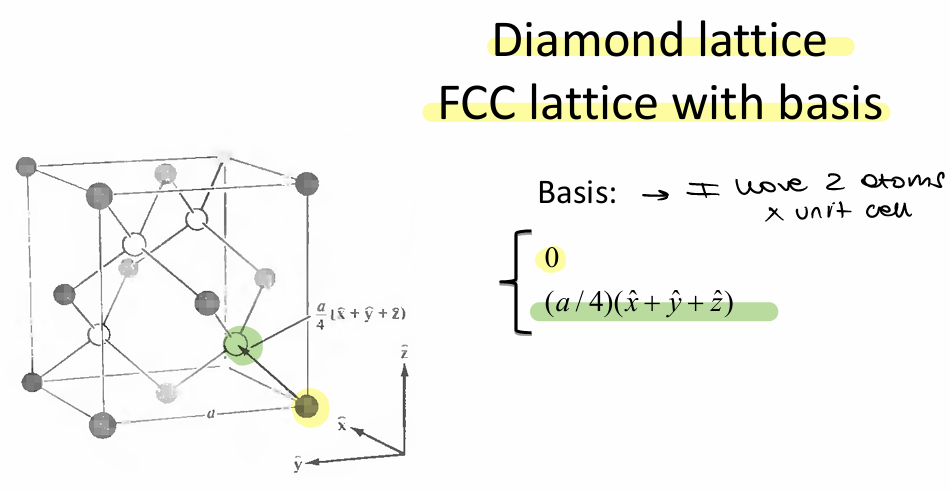
\includegraphics[width=0.9\textwidth]{images/2-Cristalli/diamantebase1.png}
	\caption{}
	\label{fig:diamantebase1}
\end{figure} 
\begin{figure} [H]
	\centering
	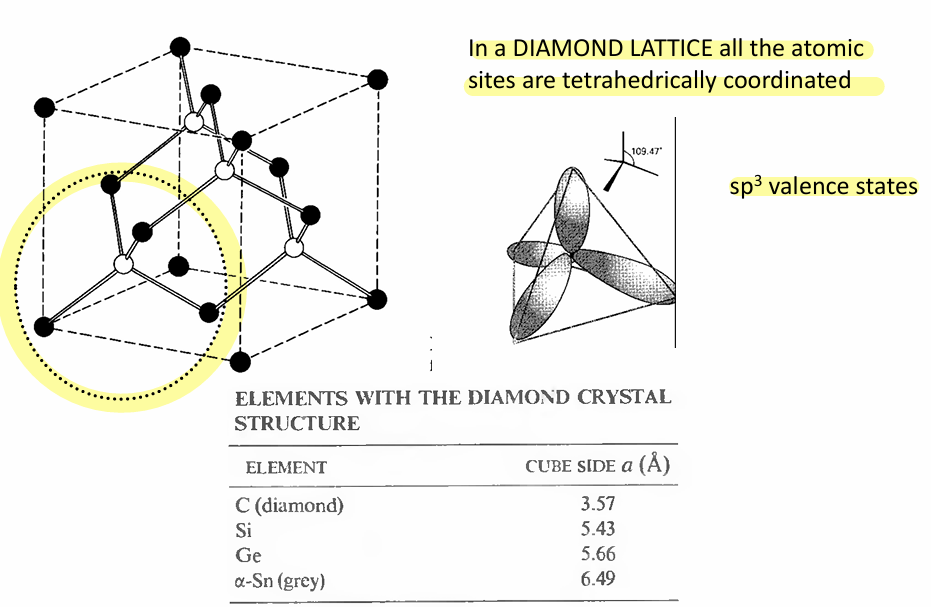
\includegraphics[width=0.9\textwidth]{images/2-Cristalli/diamantebase2.png}
	\caption{}
	\label{fig:diamantebase2}
\end{figure} 

Un altro esempio di cristallo con base che è un diamante FCC è la \textbf{zincoblenda}, in questo caso però si hanno due atomi all'interno della cella che sono diversi (esempi di cristalli sono: ZnS, CuF, CuCl ecc). Tieni a mente che non sono dei reticoli di Bravais

\subsection{Hexagonal Closed Packed Structure (HCP)}
Anche se non è un reticolo di Bravais l'HCP è una delle strutture più presenti in natura assieme ai reticoli di Bravais FCC e BCC. La struttura consiste in due reticoli di Bravais ad esagono semplice inter-penetranti spostati l'uno dall'altro di $\frac{a_1}{3}+\frac{a_2}{3}+\frac{a_3}{2}$. 
\begin{figure} [H]
	\centering
	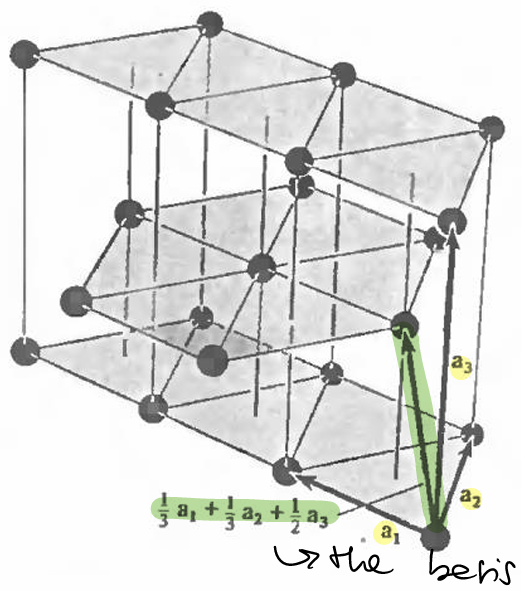
\includegraphics[width=0.35\textwidth]{images/2-Cristalli/HCP1.png}
	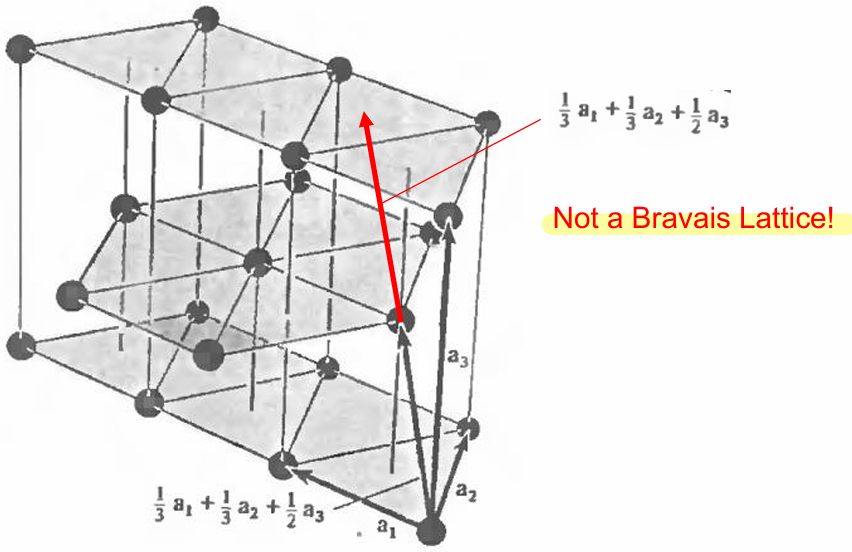
\includegraphics[width=0.55\textwidth]{images/2-Cristalli/HCP2.png}
	\caption{si può notare che l'HCP non è un reticolo di Bravais}
	\label{fig:HCP}
\end{figure} 

Si può notare che è un tipo di struttura che promuove atomi con forze isotropiche e a corto raggio (Forza di Coulumb o di Wan Der Waals), mentre atomi in cui prevale la direzionalità e forze a lungo raggio favoriscono la formazione di strutture FCC piuttosto che HCP.\\ 

\subsection{Altri reticoli con base}
\subsubsection{Struttura del cloruro di sodio}
È formato da 2 diversi atomi quindi rompo la simmetria perciò sicuramente non può essere descritto da un semplice reticolo di Bravais ma è un reticolo di Bravais FCC (quindi ha i vettori primitivi dell'FCC, e lo forma con cloro e ha il sodio all'interno della cella unitaria) con base $\frac{a}{2}(\hat{x}+\hat{y} + \hat{z})$. È un cristallo ionico, degli esempi cristalli di questa forma oltre all'NaCl sono NaF, NaI, KBr ecc...
\begin{figure} [H]
	\centering
	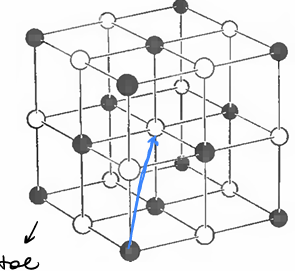
\includegraphics[width=0.35\textwidth]{images/2-Cristalli/NaCl.png}
	\caption{struttura cristallina dell'NaCl}
	\label{fig:NaCl}
\end{figure}

\subsubsection{Struttura del cloruro di cesio}
È un BCC con base $\frac{a}{2}(\hat{x}+\hat{y} + \hat{z})$ . Le forze principali in gioco sono le forze di coulomb e questa è la struttura che minimizza l'energia. Esempi di cristalli con questa struttura oltre al CsCl sono: CsBr e CsI
\begin{figure} [H]
	\centering
	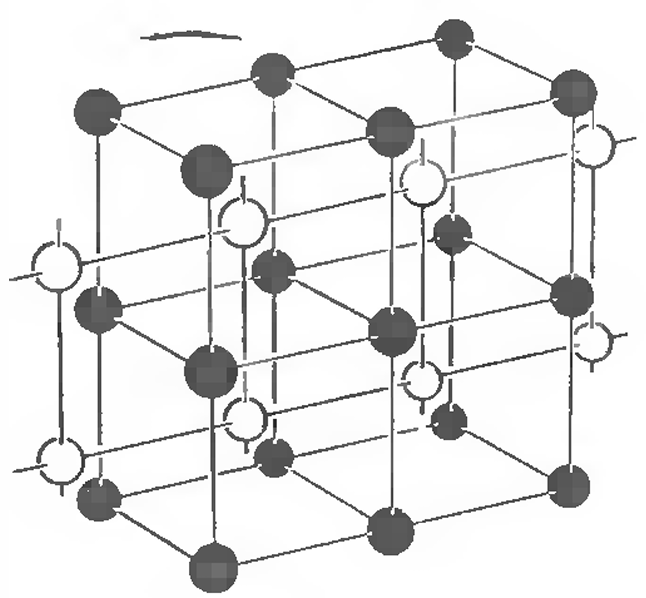
\includegraphics[width=0.35\textwidth]{images/2-Cristalli/CsCl.png}
	\caption{struttura cristallina dell'CsCl, l'atomo bianco al centro del BCC è un atomo diverso dagli altri quindi è per questo che necessito un reticolo di Bravais con base}
	\label{fig:CsCl}
\end{figure}
In poche parole se ho due atomi diversi nel cristallo sicuramente non sarà descritto da un reticolo di Bravais.


\section{Reticolo Reciproco}

Quando si eseguono esperimenti di diffrazione con raggi X per studiare la struttura cristallina, ciò che viene effettivamente osservato è la trasformata di Fourier delle posizioni degli atomi. In questo contesto, la trasformata di Fourier di un reticolo di Bravais risulta essere essa stessa un reticolo di Bravais, detto \textbf{reticolo di Bravais reciproco}.

\subsection*{Definizione di Reticolo Reciproco}

La definizione corretta è la seguente: l'insieme dei vettori d'onda \(\vec{K}\) tali che le onde piane associate \(e^{i\vec{K}\cdot \vec{r}}\) abbiano la stessa periodicità del dato reticolo di Bravais, costituisce il reticolo reciproco. In altre parole, per ogni vettore di traslazione \(\vec{R}\) del reticolo (cioè \(\vec{R}\) appartenente al reticolo di Bravais) deve valere:
\[
e^{i\vec{K}\cdot (\vec{r} + \vec{R})} = e^{i\vec{K}\cdot \vec{r}} \quad \forall\, \vec{r}.
\]
Da ciò segue che:
\[
e^{i\vec{K}\cdot \vec{R}} = 1.
\]
Pertanto, l'insieme dei vettori \(\vec{K}\) che soddisfano la condizione
\[
e^{i\vec{K}\cdot \vec{R}} = 1 \quad \text{per ogni } \vec{R} \text{ del reticolo di Bravais}
\]
definisce il reticolo reciproco.

Notiamo che se \(e^{i\vec{K}\cdot \vec{R}} = 1\) per ogni \(\vec{R}\), l'onda piana \(e^{i\vec{K}\cdot \vec{r}}\) assume lo stesso valore in tutti i punti del reticolo, cioè la funzione è periodica con la medesima periodicità del reticolo reale. In sostanza, il reticolo reciproco è costituito dai vettori \(\vec{K}\) associati ad onde piane la cui periodicità coincide con quella del reticolo di Bravais.

\subsection*{Chiusura per Addizione e Sottrazione}

Una proprietà importante del reticolo reciproco è la sua invarianza rispetto ad addizione e sottrazione. Infatti, se \( \vec{K},\, \vec{K'} \) appartengono al reticolo reciproco, allora:
\[
e^{i(\vec{K}+\vec{K'}) \cdot \vec{R}} = e^{i\vec{K}\cdot \vec{R}}\, e^{i\vec{K'}\cdot \vec{R}} = 1 \cdot 1 = 1,
\]
quindi anche \( \vec{K}+\vec{K'} \) appartiene al reticolo reciproco. Lo stesso vale per la sottrazione. Questo fatto mostra che il reticolo reciproco possiede la struttura di un reticolo di Bravais.

\subsection*{Relazione tra Reticolo di Bravais e Reticolo Reciproco}

Il reticolo reciproco permette di determinare geometricamente il reticolo di Bravais originale. Se sono dati i vettori primitivi \( \vec{a}_1, \vec{a}_2, \vec{a}_3 \) del reticolo di Bravais, i vettori primitivi del reticolo reciproco si definiscono in questo modo:
\[
\vec{b}_1 = 2\pi\, \frac{\vec{a}_2 \times \vec{a}_3}{\vec{a}_1 \cdot (\vec{a}_2 \times \vec{a}_3)},
\]
\[
\vec{b}_2 = 2\pi\, \frac{\vec{a}_3 \times \vec{a}_1}{\vec{a}_1 \cdot (\vec{a}_2 \times \vec{a}_3)},
\]
\[
\vec{b}_3 = 2\pi\, \frac{\vec{a}_1 \times \vec{a}_2}{\vec{a}_1 \cdot (\vec{a}_2 \times \vec{a}_3)}.
\]
Da queste definizioni si può dimostrare che i vettori primitivi \(\vec{b}_i\) soddisfano la relazione:
\[
\vec{b}_i \cdot \vec{a}_j = 2\pi\, \delta_{ij},
\]
dove \(\delta_{ij}\) è il delta di Kronecker.

\subsection*{Verifica della Condizione di Periodicità}

Per vedere che i vettori \(\vec{b}_i\) appartengono al reticolo reciproco, consideriamo un generico vettore di traslazione del reticolo reale:
\[
\vec{R} = n_1 \vec{a}_1 + n_2 \vec{a}_2 + n_3 \vec{a}_3 \quad \text{con } n_i \in \mathbb{Z}.
\]
Un generico vettore \(\vec{K}\) del reticolo reciproco si può scrivere come:
\[
\vec{K} = k_1 \vec{b}_1 + k_2 \vec{b}_2 + k_3 \vec{b}_3 \quad \text{con } k_i \in \mathbb{Z}.
\]
Il prodotto scalare risulta dunque:
\[
\vec{K} \cdot \vec{R} = k_1 n_1\, (\vec{b}_1 \cdot \vec{a}_1) + k_2 n_2\, (\vec{b}_2 \cdot \vec{a}_2) + k_3 n_3\, (\vec{b}_3 \cdot \vec{a}_3) = 2\pi (k_1 n_1 + k_2 n_2 + k_3 n_3).
\]
Pertanto:
\[
e^{i \vec{K}\cdot \vec{R}} = e^{i 2\pi (k_1 n_1 + k_2 n_2 + k_3 n_3)} = 1,
\]
il che dimostra che \(\vec{K}\) soddisfa la condizione di periodicità richiesta per appartenere al reticolo reciproco.

\subsection*{Correlazione tra Tipologie di Reticolo}

Un aspetto interessante è la relazione tra alcuni reticoli di Bravais e i loro reticoli reciproci. Ad esempio, si ha:
\begin{center}
	\begin{tabular}{|c|c|}
	\hline
	Reticolo di Bravais & Reticolo Reciproco \\ 
	\hline
	Simple Cubic (SC) & Simple Cubic (SC) \\
	\hline
	Face-Centered Cubic (FCC) & Body-Centered Cubic (BCC) \\
	\hline
	Body-Centered Cubic (BCC) & Face-Centered Cubic (FCC) \\
	\hline
	\end{tabular}
\end{center}
In altre parole, un cristallo con struttura FCC ha come reticolo reciproco una struttura BCC, e viceversa.


\section{Zona di Brillouin}
La \textbf{zona di Brillouin} è la cella di wigner seitz del reticolo reciproco. 
\\~\\
La \textbf{prima zona di Brillouin} è l'insieme di punti nello spazio reciproco/ k-space che possono essere raggiunti dall'origine senza attraversare nessun piano di Bragg.\\\\
La \textbf{seconda zona di Brillouin} è l'insieme di punti nello spazio reciproco che possono essere raggiunti dall'origine attraversando un solo piano di Bragg. \\\\
La $(n+1)$\textbf{-esima zona di Brilluoin} è l'insieme di punti nello spazio reciproco, che non stanno nella $(n-1)$-esima zona, che può essere raggiunto dalla n-esima zona di Brilluoin attraversando un solo piano di Bragg. \\
I \textbf{piani di Bragg} sono i piani che tagliano in due la connessione tra gli atomi.
\begin{figure} [H]
	\centering
	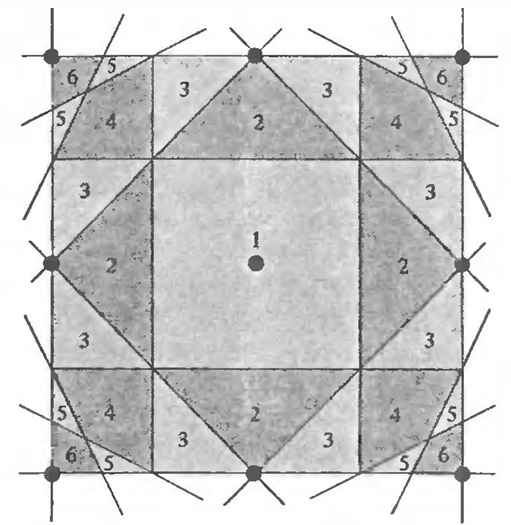
\includegraphics[width=0.4\textwidth]{images/2-Cristalli/BZ.png}
	\caption{queste sono le varie zone di Brillouin in un cristallo e i piani di Bragg sono indicati dale linee}
	\label{fig:BZ}
\end{figure}

in Figura \ref{fig:esBZ} sono riportati degli esempi dove si può osservare l'esterno di varie zone di Brillouin per reticoli FCC e BCC. Allontanandoci dal Piano di Bragg i cambiamenti della struttura elettronica sono deboli mentre vicino ai piani di Bragg sono molto forti, questo concetto è alla base dei gap nei solidi, conoscere le zone di Brillouin è fondamentale per capire la struttura elettronica e le sue interazioni.
\begin{figure} [H]
	\centering
	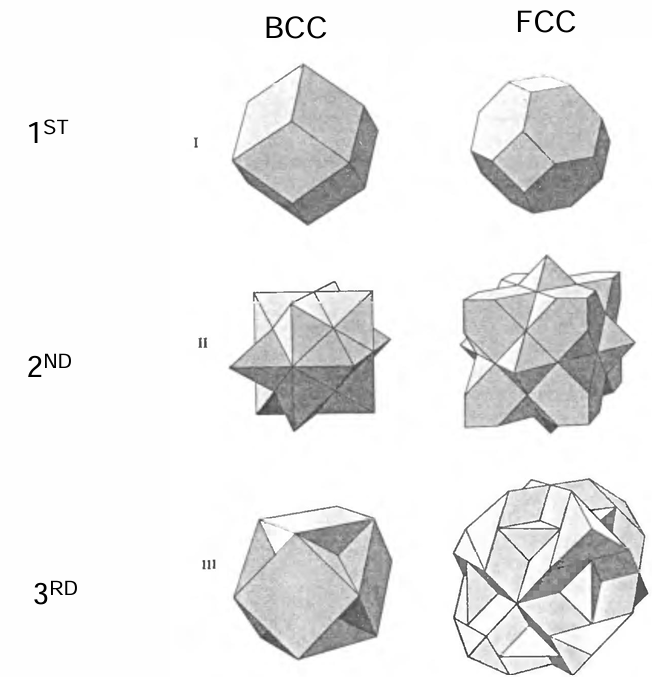
\includegraphics[width=0.45\textwidth]{images/2-Cristalli/esBZ.png}
	\caption{}
	\label{fig:esBZ}
\end{figure}
\section{Piani del reticolo}
Possiamo pensare ad un cristallo come ad una collezione di piani a distanza d, e posso identificare ogni piano con un vettore del reticolo reciproco. \\\\
Per una qualasiasi famiglia di piani cristallini separati da una distanza d, ci sono dei vettori del reticolo reciproco $\mathbf{K}$ perpendicolari al piano , il più corto sarà di lunghezza $\frac{2\pi}{d}$. \\\\
Al contrario, per un qualsiasi vettore del reticolo reciproco $\mathbf{K}$ c'è una famiglia di piani perpendicolari a $\mathbf{K}$ separati da una distanza d dove $\frac{2\pi}{d}$ è la lunghezza del vettore più corto del reticolo reciproco parallelo a K. \\\\
$k_0 = \frac{2\pi}{d}$ ha questa forma perché l'onda piana deve avere lo stesso valore nello spazio k, la dimostrazione di ciò è in Figura \ref{fig:dimpiani}
\begin{figure} [H]
	\centering
	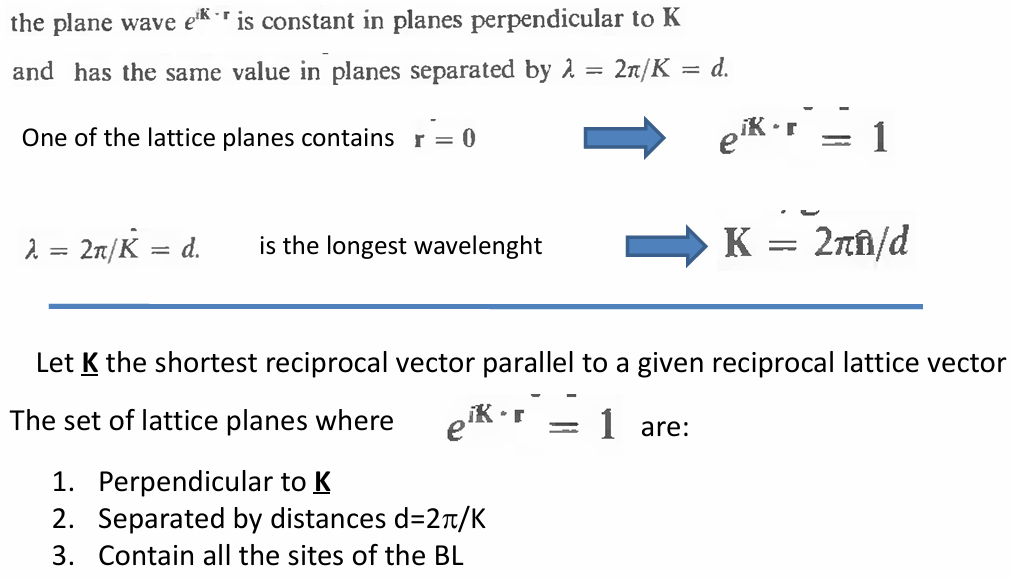
\includegraphics[width=0.9\textwidth]{images/2-Cristalli/dimpiani.png}
	\caption{}
	\label{fig:dimpiani}
\end{figure}

\subsection{Indice di Miller}
Dalla corrispondenza tra i vettori del reticolo reciproco e una famiglia di piani del cristallo possiamo definire un modo più conveniente per specificare l'orientazione del piano. L'\textbf{indice di Miller} di un piano del cristallo sono le coordinate del vettore del reticolo reciproco più corto perpendicolare a quel piano rispetto ad un set di vettori primitivi del reticolo reciproco specifico. Un piano con indici di miller h, k, l è perpendicolare ad un vetorre del reticolo reciproco $hb_1 + kb_2 + lb_3$. Quindi gli indici di Miller sono degli interi e dipendono da una particolare scelta di vettori primitivi. La definizione di indici di Miller è riportata in Figura \ref{fig:indicemiller}
\begin{figure} [H]
	\centering
	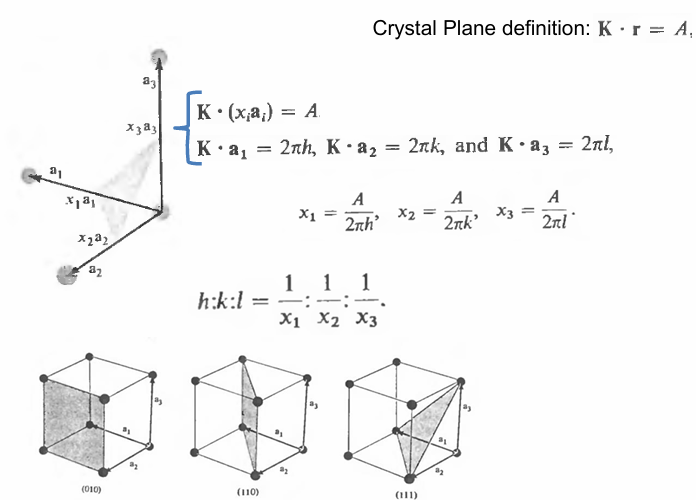
\includegraphics[width=0.9\textwidth]{images/2-Cristalli/indicemiller.png}
	\caption{}
	\label{fig:indicemiller}
\end{figure}

Ci sono diverse notazioni per indicare gli indici di miller una è (001), i piani equivalenti nello spazio reciproco sono $\{ 001 \}$ invece nel piano reale la direzione del cristallo è indicata con $[001]$ e le direzioni equivalenti con $<001>$.

\section{Diffrazione raggi-x nei cristalli e definizione della struttura cristallina}
\subsection{Formulazione di Bragg}
La formulazione di Bragg è un modello che descrive la diffrazione dei raggi X (o di altre onde) da parte di un cristallo, basandosi sull'idea che il cristallo sia costituito da piani reticolari paralleli composti da ioni separati da una distanza $d$ che agiscono come superfici riflettenti.\\\\
Quando un fascio di raggi X incide su un cristallo, esso può essere parzialmente riflesso da strati atomici interni.  L'obbiettivo è comprendere e studiare la posizione dei piani che compongono il solido osservando gli spot generati dalla diffrazione con i raggi X. \\\\
La condizione per cui questi raggi riflessi interferiscono in modo costruttivo è data dalla legge di Bragg:
\[2d\sin\theta = n\lambda\]
con $\theta$ angolo di incidenza detto di Bragg, $n$ numero intero. \\\\
\begin{figure} [H]
	\centering
	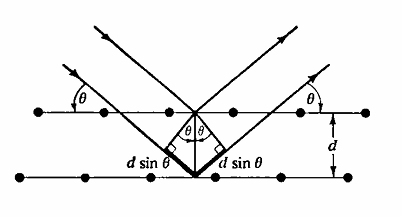
\includegraphics[width=0.4\textwidth]{images/2-Cristalli/braggdiffr.png}
	\caption{rappresentazione grafica della diffrazione, $d\sin \theta$ è la differenza di cammino ottico tra i due raggi riflessi sui diversi piani che determinerà quindi una differenza di fase}
	\label{fig:braggdiffr}
\end{figure}
Limiti:
\begin{itemize}
    \item È una descrizione semplificata che considera il cristallo come una serie di piani paralleli senza tenere conto dell'effetto della diffrazione su scala atomica più fine.
    \item Non include effetti come l'assorbimento dei raggi X o le anomalie legate alla dispersione.
    \item Siccome i piani hanno diverse direzioni ci sarebbe più un $\theta$ da prendere in considerazione.
\end{itemize}



\subsection{Formulazione di Von Laue}
\label{subsec:Formulazione-di-Von-Laue}
IPOTESI:
\begin{enumerate}
    \item Non viene individuata nessuna particolare suddivisione in piani reticolari e non viene imposta nessuna ipotesi di riflessione speculare, ossia non si assume che ogni raggio diffuso da un punto di scattering interferisca in modo costruttivo.\\
    \item Il reticolo è composto da oggetti macroscopici identici posti su dei siti in posizione $\vec{R}$ del B.L. e ciascuno ri-irradia la radiazione in tutte le direzioni.\\
\end{enumerate}
Per ottenere le condizioni di interferenza costruttiva considero uno scattering elastico come in Figura \ref{fig:vonform}, ossia supponiamo che un fascio di raggi X incida su 2 scatteratori posti a distanza $\vec{d}$ con $k$ vettore d'onda incidente e $k'$ vettore d'onda riflesso. 
\begin{figure} [H]
	\centering
	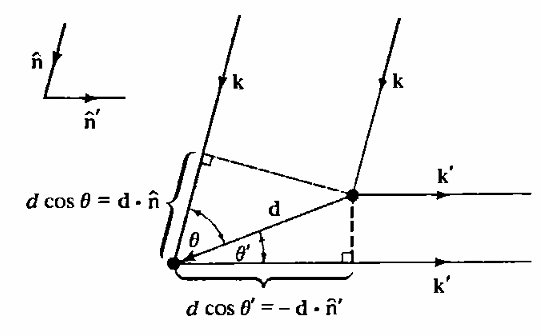
\includegraphics[width=0.5\textwidth]{images/2-Cristalli/vonform.png}
	\caption{}
	\label{fig:vonform}
\end{figure} 

La differenza di cammino ottico è data da:
\[ d\cos \theta + d \cos\theta' = d \cdot (\hat{n} - \hat{n}')\] 
e la condizione per ottenere interferenza costruttiva è:
\[ d \cdot ( \hat{n} - \hat{n}') = m\lambda  \]
siccome lo scattering è elastico avremo che $|k| = |k'|$, moltiplicando da entrambe le parti per $|k| = \frac{2\pi \hat{n}}{\lambda}$ ottengo: 
\[ d \cdot (k - k') = 2\pi m \implies R \cdot (k - k') = 2\pi m \]
poiché d è un vettore del reticolo di reciproco. Quindi guardando ai diversi spot della diffrazione posso ottenere informazioni sul reticolo di Bravais quindi
\[ e^{i(k'-k) \cdot R} = 1\]
confrontando questo risultato con la definizione di reticolo reciproco che è \\ $e^{i K \cdot R} = 1$ arriviamo alla \textbf{condizione di Laue che dice che l'interfenza costruttiva compare provocando un cambiamento nel vettore d'onda pari a $K = k'-k$ che è un vettore del reticolo reciproco}.


Nella condizione in cui $k$ e $k'$ sono uguali prendo $ |k| = |k-K|$ e facendo al quadrato entrambe le parti otteniamo: (ovviamente sono tutti vettori)
\[ \cancel{k^2} =\cancel{ k^2 }+ K^2 - 2k \cdot K \implies  2\vec{k} \cdot \vec{K} = K^2  \implies \frac{1}{K} 2k \cdot K = K^2 \frac{1}{K} \implies \vec{k} \cdot \hat{K} = \frac{1}{2} K\]
\textbf{La componente del vettore incidente k lungo il vettore del reticolo reciproco K deve essere metà della lunghezza di K.}\\\\
La formulazione di Laue è particolarmente utile quando si analizzano pattern di diffrazione complessi, specialmente con sorgenti policromatiche, in cui sono presenti molteplici lunghezze d’onda.
\begin{figure} [H]
	\centering
	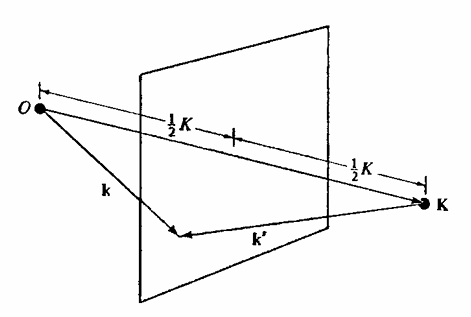
\includegraphics[width=0.5\textwidth]{images/2-Cristalli/vonlaue2.png}
	\caption{}
	\label{fig:vonlaue2}
\end{figure} 

\subsubsection{Equivalenza tra Von Laure e Bragg}
L'equivalenza tra i due criteri segue dalla relazione tra i vettori del reticolo reciproco e le famiglie di piani del cristallo. \\\\
Si supponga che il vettore d'onda incidente k e k' soddisfino la condizione di Laue che dice che $K = k'-k$ è un vettore del reticolo reciproco. Si nota dalla Figura \ref{fig:VLBeq} che k e k' hanno lo stesso angolo $\theta$ con il piano perpendicolare a K. \\
Quindi lo scattering può essere visto come una riflessione di Bragg, con un angolo di Bragg $\theta$ dalla famiglia di piani perpendicolari al vettore del reticolo reciproco K.
\begin{figure} [H]
	\centering
	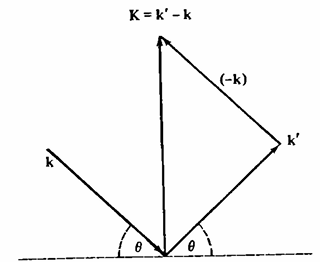
\includegraphics[width=0.5\textwidth]{images/2-Cristalli/VLBeq.png}
	\caption{}
	\label{fig:VLBeq}
\end{figure} 

Per dimostrare che questa affermazione soddisfi la condizione di Bragg, si noti che K è multiplo del vettore del reticolo reciproco più corto parallelo a $\mathbf{K} $
\[\implies K = n K_0 \hspace{0.3cm} \text{siccome} K_0 = \frac{2\pi}{d}\hat{n} \implies K = \frac{2\pi n}{d}\]
Dalla Figura \ref{fig:VLBeq} si osserva anche che $K = 2k \sin \theta$ perciò vale:
\[ k \sin \theta = \frac{\pi n}{d}, \ \ k = \frac{2\pi}{\lambda} \implies n\lambda = 2d\sin \theta \]
Questo significa che Bragg e Von Laue sono equivalenti. \textbf{Quindi la diffrazione di Laue corrisponde ad un cambio nel vettore d'onda dato da un vettore $\mathbf{K}$ del reticolo reciproco che corrisponde ad una riflessione di Bragg da una famiglia di piani del reticolo perpendicolari a \textbf{K}}.

\section{Costruzione di Ewald e metodo di Laue}
Una volta che ho i picchi di diffrazione posso ricostruire la struttura del cristallo ed un modo per farlo è utilizzando il metodo di Ewald che si può osservare in Figura \ref{fig:ewald}, grazie a questo strumento grafico si possono vedere immediatamente quali direzioni del reticolo (cioè quali piani interni al cristallo) genereranno riflessioni costruttive.\\\\
Si disegna una sfera (chiamata sfera di Ewald) con raggio $r = \frac{1}{\lambda} = k$, il centro della sfera è posto alla punta del vettore $k$.
I punti del reticolo reciproco che cadono sulla superficie di questa sfera sono quelli che soddisfano la condizione di diffrazione, siccome non ho mai un fascio monocromatico di Raggi X, ho più spot e quindi delle lunghezze d'onda comprese in un certo intervallo $\lambda_1 < \lambda < \lambda_0$.\\\\
Posso quindi usare i corrispondenti $k_{min}$ e $k_{max}$ per disegnare il cerchio come quello in Figura \ref{fig:metVL}, i picchi di Bragg saranno osservati per ogni vettore del reticolo reciproco compreso nelle sfere di Ewald di raggio $k_1$ e $k_0$.
\begin{figure} [H]
	\centering
	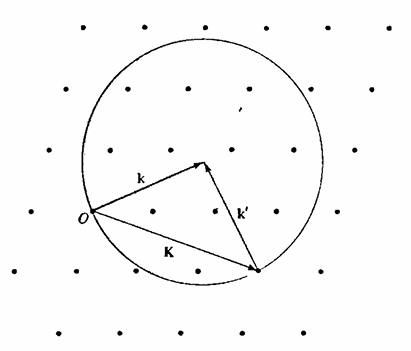
\includegraphics[width=0.5\textwidth]{images/2-Cristalli/ewald.png}
	\caption{}
	\label{fig:ewald}
\end{figure} 
\begin{figure} [H]
	\centering
	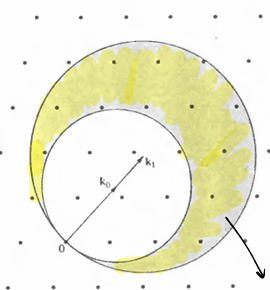
\includegraphics[width=0.5\textwidth]{images/2-Cristalli/metVL.png}
	\caption{L'interferenza si osserverà solo per i punti all'interno dell'area colorata}
	\label{fig:metVL}
\end{figure}

Ruotando il cristallo, ruoto anche il reticolo reciproco, alcuni punti che prima della rotazione non intersecavano la sfera di Edwald in seguito potrebbero farlo (come si osserva in Figura \ref{fig:esEd}) quindi ricostruendo di quanto il cristallo è stato ruotato vedo punti apparire e sparire e posso ricostruire il reticolo reciproco e quindi tornando allo spazio reale descrivere l'orientamento e la simmetria del cristallo.
\begin{figure} [H]
	\centering
	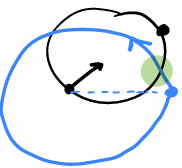
\includegraphics[width=0.3\textwidth]{images/2-Cristalli/esEd.png}
	\caption{Senza ruotare il cristallo il punto considerato non avrebbe intersecato la sfera di edwald}
	\label{fig:esEd}
\end{figure}

\section{Fattore di struttura geometrica }
Possiamo avere la prova che un reticolo sia un reticolo di Bravais semplice oppure uno con base osservando i raggi X? \\
Se è con base l'intensità dei punti non sarà la stessa e questo è dovuto alla presenza del \textbf{fattore geometrico} che è:
\[ S_k = \sum_{j =1}^n e^{i K \cdot d_j} \]
dove j è la posizione dell'atomo, $S_k$ che dipende da K è l'effetto dell'interferenza tra i fasci di raggi X scatterati dal primo e dal secondo atomo, infatti l'intensità del picco cambia con K ed è data da $|S_k|^2$. I raggi x sono la superposizione della diffrazione degli atomi per cella unitaria, negli altri casi c'è interferenza tra 2 atomi della cella. Vedo una modulazione che dipende dalla posizione dei due atomi. \\\\
Ora proviamo a calcolare il Fattore di struttura geometrica per per un BCC considerato come un SC con base riportato in Figura \ref{fig:BCCSC}.
\begin{figure} [H]
	\centering
	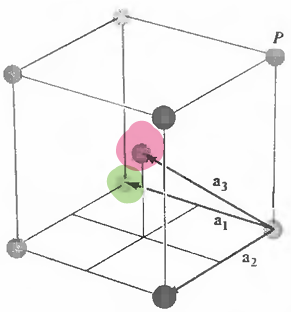
\includegraphics[width=0.3\textwidth]{images/2-Cristalli/BCCSC.png}
	\caption{i punti evidenziati sono $d_1$ e $d_2$}
	\label{fig:BCCSC}
\end{figure}
$d_1 = (0,0,0)$ è il punto nell'angolo mentre $d_2 = \frac{a}{2}(\hat{x}+\hat{y}+\hat{z})$ i vettori del reticolo sono $\Vec{K} = \frac{2\pi}{a}(n_1 \hat{x} + n_2 \hat{y} + n_3 \hat{z})$ per ogni punto del reticolo il fattore di struttura è:
\[ S_k = \sum e^{i \Vec{K}\cdot d_i} = 1 + \exp[i\Vec{K} \cdot \frac{1}{2}(\hat{x}+\hat{y}+\hat{z})] \]
Nel caso in cui i due atomi fossero diversi posso aggiungere un termine $\eta$ 
\[ S_k = 1 +\eta e^{i \pi(n_1 + n_2 + n_3)} = 1 + \eta(-1)^{n_1 + n_2 + n_3} = 
\begin{cases}
1+ \eta, \ n_1 + n_2 + n_3 \ \text{pari} \\
1-\eta, \ n_1 + n_2 + n_3  \ \text{dispari}
\end{cases} \]
Quindi a seconda del punto k ho un'intensità diversa. \\
Invece in un cristallo poliatomico gli ioni nella base non sono identici e quindi ciò che dovrebbe essere $\eta(K)$ dipende da K, quindi il fattore di struttura è:
\[ S_k = \sum_{j = 1}^n f_i(\Vec{K})e^{i K \cdot d_j}  \]
$f_j(K)$ è detto fattore di forma atomica ed è dato da:
\[ f_j(\Vec{K}) = -\frac{1}{e}\int  e^{i \Vec{K} \cdot \Vec{r}} \rho_j(r)\ \d\Vec{r} \]
ed è praticamente la trasformata di Fourier della densità di carica dell'atomo. \\\\
